Rätselaufgabe: Es geht die Rede, dass drei Nachbarn, die gemeinsam einen kleinen Park hatten, so wie im Bild zu sehen ist, Streit bekamen. Der Besitzer des großen Hauses beklagte sich über die Hühner seiner Nachbarn, die ihn störten, und baute von seiner Tür zum Tor vorn im Bild einen abgegrenzten Weg. Daraufhin baute der Mann in dem Haus rechts einen Weg zum Tor auf der linken Seite und der Mann in dem Haus links einen Weg zum Tor auf der rechten Seite.
Die Wege kreuzten sich an keiner Stelle. Können Sie alle drei richtig einzeichnen?

\begin{figure}[ht]
	\centering
  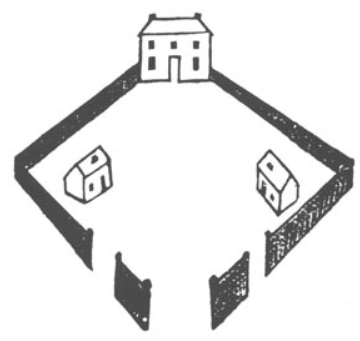
\includegraphics[width=0.3\textwidth]{../tex-snippets/ex-graph-theory-1-img-a.png}
%	\caption{}
	\label{fig1}
\end{figure}

